\RequirePackage{lineno}
\documentclass[twocolumn,preprintnumbers,amsmath,amssymb,superscriptaddress]{revtex4}
%\usepackage[pdftex]{graphicx}

\usepackage{amsmath,amsfonts,amssymb}
\usepackage[english]{babel}
\usepackage[latin1]{inputenc}
\usepackage[T1]{fontenc}
\usepackage{color}
\usepackage{float}
\usepackage{verbatim}
\usepackage{graphicx}
\usepackage{bm}
\usepackage{mathtools}
\usepackage{stmaryrd}
\usepackage{anyfontsize}


%\usepackage{epstopdf}
%\usepackage{array}
%\usepackage{tabularx}
%\usepackage{multirow}
\usepackage{color}
%\usepackage{multibox}
%\usepackage{rotating}
%\usepackage{lineno}
%\usepackage[left]{lineno}
\usepackage[comma,sort&compress]{natbib}
\bibpunct{}{}{,}{s}{}{;}
%\usepackage{authblk}
%\usepackage{multicol}

\bibliographystyle{naturemag}

% \usepackage{bibunits}

\linenumbers
 \setlength\linenumbersep{3pt}
 
\addto\captionsenglish{\renewcommand{\figurename}{Figure S\!}}

\begin{document}


\author{Justin D. Yeakel} \affiliation{School of Natural Sciences, University
  of California, Merced, Merced, CA 95340, USA}\affiliation{The Santa Fe Institute, 1399 Hyde Park Road, Santa Fe, NM 87501, USA}\affiliation{Contributed equally}\affiliation{Corresponding author}

\author{Christopher P. Kempes} \affiliation{The Santa Fe Institute, 1399 Hyde
  Park Road, Santa Fe, NM 87501, USA}\affiliation{Contributed equally}\affiliation{Corresponding author}

\author{Sidney Redner} \affiliation{The Santa Fe Institute, 1399 Hyde Park
  Road, Santa Fe, NM 87501, USA}\affiliation{Contributed equally}\affiliation{Corresponding author}

\title{ Supporting Information for ``The dynamics of starvation and recovery''}%: Eco-evolutionary feedbacks}



\maketitle


%%%%%%%%%%%%%%%%%%%%%%%%
% SUPPLEMENTARY MATERIAL
%%%%%%%%%%%%%%%%%%%%%%%%

%New additions in red text


\clearpage

{\bf Mechanisms of Starvation and Recovery}
To understand the dynamics of starvation, recovery, reproduction, and resource competition, our framework partitions consumers into two classes: (a) a full class that is able to reproduce and, (b) a hungry class that experiences mortality at a given rate and is unable to reproduce. For the dynamics of growth, reproduction, and resource consumption, past efforts have combined the overall metabolic rate, as dictated by body size, with a growth rate that is dependent on resource abundance and, in turn, dictates resource consumption (see Refs. \citep{Kempes:2012hy,kempes2014morphological} for a brief review of this perspective). This approach has been used to understand a range of phenomena including a derivation of ontogenetic growth curves from a partitioning of metabolism into maintenance and biosynthesis (e.g. \citep{West:2001bv,moses2008rmo,hou,Kempes:2012hy}) and predictions for the steady-state resource abundance in communities of cells \citep{kempes2014morphological}. Here we leverage these mechanisms, combined with several additional concepts, to define our Nutritional State Model (NSM).

We consider the following generalized set of explicit dynamics for starvation, recovery, reproduction, and resource growth and consumption
\begin{align}
\begin{split}
\dot{F_{d}} &= \lambda_{\text{max}} F_{d} + \rho_{\text{max}}R_{d}H_{d}/k - \sigma \left(1-\frac{R_{d}}{C}\right)F_{d},  \\
\dot{H_{d}} &= \sigma \left(1-\frac{R_{d}}{C}\right)F_{d} - \rho_{\text{max}}R_{d} H_{d}/k - \mu H_{d},  \\
\dot{R_{d}} &= \alpha R_{d}\left(1-\frac{R_{d}}{C}\right) -\\
& \left[\left(\frac{\rho_{\text{max}}R_{d}}{Y_{H}k}+P_{H}\right)H_{d}+\left(\frac{\lambda_{\text{max}}}{Y_{F}}+P_{F}\right)F_{d}\right].
\label{bigdynamics}
\end{split}
\end{align}
where each term has a mechanistic meaning that we detail below (we will denote the dimensional equations with the subscript $_{d}$ before introducing the non-dimensional form that is presented in the main text). In the above equations $Y$ represents the yield coefficient (e.g., Refs. \citep{pirt,Heijnen}) which is the quantity of resources required to build a unit of organism (gram of mammal produced per gram of resource consumed) and $P$ is the specific maintenance rate of resource consumption (g resource $\cdot$ s$^{-1}$ $\cdot$ g organism$^{-1}$). If we pick $F_{d}$ and $H_{d}$ to have units of (g organisms $\cdot$ m$^{-2}$), then all of the terms of $\dot{R_{d}}$, such as $\frac{\rho\left(R_{d}\right)}{Y}H_{d}$, have units of (g resource $\cdot$ m$^{-2}$ $\cdot$ s$^{-1}$) which are the units of net primary productivity (NPP), a natural choice for $\dot{R_{d}}$. This choice also gives $R_{d}$ as (g $\cdot$ m$^{-2}$) which is also a natural unit and is simply the biomass density. In these units $\alpha$ (s$^{-1}$) is the specific growth rate of $R_{d}$, $C$ is the carrying capacity, or maximum density, of $R_{d}$ in a particular environment, and $k$ is the half-saturation constant (half the density of resources that would lead to maximum growth).
%(note this is not fully explicit because I don't know how to deal with the response of $\sigma$ to resources, although I have an idea for a derivation which may be necessary given the following approximations)




%\begin{align}
%\begin{split}
%\dot{F_{d}} &= \lambda\left(R_{d}\right) F_{d} + \rho\left(R_{d}\right)H_{d} - \sigma \left(1-\frac{R_{d}}{C}\right)F_{d},  \\
%\dot{H_{d}} &= \sigma \left(1-\frac{R_{d}}{C}\right)F_{d} - \rho\left(R_{d}\right)H_{d} - \mu H_{d},  \\
%\dot{R_{d}} &= \alpha R_{d}\left(1-\frac{R_{d}}{C}\right) - \\
%&\left[\left(\frac{\rho\left(R_{d}\right)}{Y}+P_{H}\right)H_{d}+\left(\frac{\lambda\left(R_{d}\right)}{Y}+P_{F}\right)F_{d}\right],
%\end{split}
%\end{align}
%
%In this set of equations $\lambda\left(R_{d}\right)$ and $\rho\left(R_{d}\right)$ are the growth and recovery rates as functions of the current resource availability. Typically these can be written as $\lambda\left(R_{d}\right)=\lambda_{max}S\left(R_{d}\right)$ or $\lambda\left(R_{d}\right)=\lambda_{max}S\left(R_{d}\right)$ where $\lambda_{max}$ and $\rho_{max}$ are the maximum growth and recovery rates respectively, which scale with body size as discussed later, and $S\left(R_{d}\right)$ is a saturating function of resources. The saturating function could, for example, be a Michaelis-Menten or Monod function of the form $\frac{R_{d}}{k+R_{d}}$, where $k$ is the half-saturation constant.
%A simplified version of the Michaelis-Menten or Monod functional form, which captures the essential features, is a linear function that saturates to a constant value above a certain abundance of $R_{d}$.
%
%Before describing the values of each of these constants, and a general non-dimensionalization of the system of equations, it is important to consider the resource regimes associated with the above equations which lead to a simplification. As discussed above, the resource saturation function should be defined by a linear regime proportional to $R_{d}$ when $R_{d}<<k$, and a constant value for $R_{d}>>k$. Thus for hungry individuals, $H_{d}$, where $R_{d}<<k$, we have that $\rho\left(R_{d}\right)\approx\rho_{max}R_{d}/k$, and for the full class, $F_{d}$, of organisms $\lambda\left(R_{d}\right)\approx\lambda_{max}$, such that the above relationships reduce to





%where $\beta=\frac{\lambda_{max}}{Y_{F}}+P$ which is just a constant that depends on the size of an organisms via the allometries for $\lambda_{max}$ and $P$ discussed later.

We can formally non-dimensionalize this system by the rescaling of $F=fF_{d}$, $H=fH_{d}$, $R=qR_{d}$, $t=st_{d}$, in which case our system of equations becomes
%(ignoring the $\sigma (1-R)F$ terms which I don't have a dimensional form for yet),:
\begin{align}
\begin{split}
&\dot{F} = \frac{1}{s}\left[\lambda_{\text{max}} F + \rho_{\text{max}}\frac{R}{qk}H - \sigma \left(1-\frac{R}{qC}\right)F\right],  \\
&\dot{H} = \frac{1}{s}\left[\sigma \left(1-\frac{R}{qC}\right)F - \rho_{\text{max}}\frac{R}{qk} H - \mu H\right],  \\
& \dot{R} = \\
&\frac{1}{s}\left[\alpha R\left(1-\frac{R}{qC}\right) -\frac{q}{f}\left[\left(\frac{\rho_{\text{max}}R}{Y_{H}kq}+P_{H}\right)H+\left(\frac{\lambda_{\text{max}}}{Y_{F}}+P_{F}\right)F\right]\right].
\end{split}
\end{align}
If we make the natural choice of $s=1$, $q=1/C$, and $f=1/Y_{H}k$, then we are left with
\begin{align}
\begin{split}
\dot{F} &= \lambda F + \xi \rho RH - \sigma \left(1-R\right)F,  \\
\dot{H} &= \sigma \left(1-R\right)F - \xi \rho RH - \mu H,  \\
\dot{R} &= \alpha R\left(1-R\right) -\left(\rho R+\delta\right)H-\beta F
\label{reduceddynamics}
\end{split}
\end{align}
where we have dropped the subscripts on $\lambda_{\text{max}}$ and $\rho_{\text{max}}$ for simplicity, and $\xi\equiv C/k$, $\delta\equiv Y_{H}kP_{H}/C$, and $\beta\equiv Y_{H}k\left(\frac{\lambda_{\text{max}}}{Y_{F}}+P_{F}\right)/C$. The above equations represent the system of equations presented in the main text.
\\

{\bf Parameter Values and Estimates}
All of the parameter values employed in our model have either been directly measured in previous studies or can be estimated from combining several previous studies. Below we outline previous measurements and simple estimates of the parameters.

Metabolic rate has been generally reported to follow an exponent close to $\eta=0.75$ (e.g., Refs. \citep{West:2001bv,moses2008rmo} and the supplement for Ref. \citep{hou}). We make this assumption in the current paper, although alternate exponents, which are known to vary between roughly $0.25$ and $1.5$ for single species \citep{moses2008rmo}, could be easily incorporated into our framework, and this variation is effectively handled by the $20\%$ variations that we consider around mean trends. The exponent not only defines several scalings in our framework, but also the value of the metabolic normalization constant, $B_{0}$, given a set of data.  For mammals the metabolic normalization constant has been reported to vary between $0.018$ (W g$^{-0.75}$) and $0.047$ (W g$^{-0.75}$; Refs. \citep{hou,West:2001bv}, where the former value represents basal metabolic rate and the latter represents the field metabolic rate. We employ the field metabolic rate for our NSM model which is appropriate for active mammals (Table 1).

An important feature of our framework is the starting size, $m_{0}$, of a mammal which adjusts the overall timescales for reproduction. This starting size is known to follow an allometric relationship with adult mass of the form $m_{0}=n_{0}M^{\upsilon}$ where estimates for the exponent range between $0.71$ and $0.94$ (see Ref. \citep{peters1986ecological} for a review). We use $m_{0}=0.097M^{0.92}$ \citep{blueweiss1978relationships} which encompasses the widest range of body sizes \citep{peters1986ecological}.

The energy to synthesize a unit of biomass, $E_{m}$, has been reported to vary between $1800$ to $9500$ (J g$^{-1}$) (e.g. Refs. \citep{West:2001bv,moses2008rmo,hou}) in mammals with a mean value across many taxonomic groups of $5,774$ (J g$^{-1}$) \citep{moses2008rmo}. The unit energy available during starvation, $E^{\prime}$, could range between $7000$ (J g$^{-1}$), the return of the total energy stored during ontogeny \citep{hou} to a biochemical upper bound of $E^{\prime}=36,000$ (J g$^{-1}$) for the energetics of palmitate \citep{stryer,hou}. For our calculations we use the measured value for bulk tissues of $7000$ which assumes that the energy stored during ontogeny is returned during starvation \citep{hou}.

For the scaling of body composition it has been shown that fat mass follows $M_{\rm fat}=f_{0}M^{\gamma}$, with measured  relationships following  $0.018M^{1.25}$ ~\citep{Dunbrack:1993ec}, $0.02M^{1.19}$ ~\citep{Lindstedt:1985hm}, and $0.026M^{1.14}$ ~\citep{Lindstedt:2002td}. We use the values from \citep{Lindstedt:1985hm} which falls in the middle of this range. Similarly, the muscle mass follows $M_{\rm musc}=u_{0}M^{\zeta}$ with $u_{0}=0.383$ and $\zeta=1.00$ ~\citep{Lindstedt:2002td}.

%We also connect the resource growth rate to the total metabolic rate of an organism. That is, we are interested in the relative rates of resource recovery and consumption by the total population. From \citep{allen2002global} the total resource use of a population with an individual body size of $M$ is given by $B_{pop}=0.00061x^{-0.03}$ (W m$^{-2}$). Considering an energy density of $18200$ (J g$^{-1}$) of grass \citep{estermann} and an NPP between and $1.59\times10^{-6}$ and $7.92\times10^{-5}$ (g s$^{-1}$ m$^{-2}$) would give a range of resource rates between  $0.029$ and $1.44$ (W m$^{-2}$). This gives a ratio of total resource consumption to supply rates between $0.00042$ and $0.021$, and we used a value of $0.002$ in our calculations and simulations.

Typically the value of $\xi=C/k$ should roughly be $2$. The value of $\rho$, $\lambda$, $\sigma$, and $\mu$ are all simple rates (note that we have not rescaled time in our non-dimensionalization) as defined in the maintext. Given that our model considers transitions over entire stages of ontogeny or nutritional states, the value of $Y$ must represent yields integrated over entire life stages. Given an energy density of $E_{d}=18200$ (J g$^{-1}$) for grass \citep{estermann} the maintenance value is given by $P_{F}=B_{0}M^{3/4}/ME_{d}$, and the yield for a full organism will be given by $Y_{F}=ME_{d}/B_{\lambda}$ (g individual $\cdot$ g grass $^{-1}$), where $B_{\lambda}$ is the lifetime energy use for reaching maturity given by
\begin{equation}
B_{\lambda}=\int_{0}^{t_{\lambda}}B_{0}m\left(t\right)^{\eta}dt.
\end{equation}
Similarly, the maintenance resource consumption rate for hungry individuals is $P_{H}=B_{0}(\epsilon_{\sigma}M)^{3/4}/(\epsilon_{\sigma}M)E_{d}$, and the yield for hungry individuals (representing the cost on resources to return to the full state) is given by $Y_{H}=ME_{d}/B_{\rho}$ where
\begin{equation}
B_{\rho}=\int_{\tau\left(\epsilon_{\sigma}\epsilon_{\lambda}\right)}^{t_{\lambda}}B_{0}m\left(t\right)^{\eta}dt.
\end{equation}
Taken together, these relationships allow us to calculate $\rho$, $\delta$, and $\beta$.

Finally, the value of $\alpha$ can be roughly estimated by the NPP divided by the corresponding biomass densities. From the data in Ref. \citep{michaletz2014convergence} we estimate the value of $\alpha$ to range between $2.81\times10^{-10}$ (s$^{-1}$) and $2.19\times10^{-8}$ (s$^{-1}$) globally. It should be noted that the value of $\alpha$ sets the overall scale of the $F^{*}$ and $H^{*}$ steady states along with $B_{tot}$ for each type. As such, we use $\alpha$ as our fit parameter to match these steady states with the data from Damuth \citep{damuth1987interspecific}. We find that the best fit is $\alpha=9.45\times10^{-9}$ (s$^{-1}$) which compares well with the calculated range above. However, two points are important to note here: first, our framework predicts the overall scaling of $F^{*}$ and $H^{*}$ independently of $\alpha$ and this correctly matches data, and second, both the asymptotic behavior and slope of $F^{*}$ and $H^{*}$ are independent of $\alpha$, such that our prediction of the maximum mammal size does not depend on $\alpha$.
\\
%For the growth rate $\lambda$ we consider the standard model of $\ln\left(\upsilon\right)/t_{\lambda}$

%More complicated models of fecundity (which, for example, account for the average length of adulthood and the number of individuals produced over this span) could be employed. However, the scaling of population growth rate has been studied in detail before and follows a relationship of $$ which matches the theory well for $\phi=.95$ and $=$.

%In our calculations we include $20\%$ variation around this value which could account for differences in efficiency during



 \begin{table}[h]
\caption{Parameter values for mammals}
\label{param}
    \begin{center}
    \footnotesize
     \begin{tabular}{p{3.8cm} c p{2.2cm} p{1.4cm}}
     \hline
    
     Definition & Parameter & Value & References  \\
     \hline
   Asymptotic adult mass & $M$ & (g) &  \\
   Initial mass of an organism & $m_{0}$ & (g) &  \\
   Metabolic rate scaling exponent & $\eta$ & $3/4$  &  (e.g. \citep{West:2001bv,moses2008rmo,hou}) \\
   Metabolic Normalization Constant & $B_{0}$ & $0.047$ (W g$^{-0.75}$)    & \citep{hou}  \\
   Initial mass scaling exponent & $\upsilon$ & $0.92$ &  \citep{blueweiss1978relationships,peters1986ecological} \\
   Initial mass scaling normalization constant & $n_{0}$ & $0.097$ (g$^{1-\upsilon}$) & \citep{blueweiss1978relationships,peters1986ecological}  \\   
   Fat mass scaling exponent & $\gamma$ & $1.19$ & \citep{Lindstedt:1985hm} \\
   Fat scaling normalization constant & $f_{0}$ & $0.02$ (g$^{1-\eta}$) & \citep{Lindstedt:1985hm}\\
   Muscle mass scaling exponent & $\zeta$ & $1.00$  & \citep{Lindstedt:2002td} \\
   Muscle scaling normalization constantv& $u_{0}$ & $0.38$ (g$^{1-\zeta}$)  & \citep{Lindstedt:2002td} \\
   Energy to synthesis a unit of mass & $E_{m}$ & $5774$ (J gram$^{-1}$)  &  \citep{moses2008rmo,West:2001bv,hou} \\
   Energy to synthesis a unit of mass during recovery & $E_{m}^{\prime}$ & $7000$ (J gram$^{-1}$) & \citep{stryer,hou} \\
   Specific resource growth rate & $\alpha$ & $9.45\times10^{-9}$ (s$^{-1}$) & see text  \\
   Fraction of asymptotic mass representing full state & $\epsilon_{\lambda}$ & $0.95$ & \citep{West:2001bv}  \\
   Fraction of asymptotic mass representing starving state & $\epsilon_{\sigma}$ & $1-f_{0}M^{\gamma-1}$ & see text  \\
   Fraction of asymptotic mass representing death & $\epsilon_{\mu}$ & $1-\frac{f_{0}M^{\gamma}+u_{0}M^{\zeta}}{M}$ & see text \\
   Carrying capacity (maximum density) of resources & $C$ & (g m$^{-2}$) & \\
   Half Saturation Constant & $k$ & (g m$^{-2}$) &   \\
   Normalized carrying capacity & $\xi$ & $C/k\approx2$ &   \\
   Reproductive fecundity & $\nu$ & $2$ & \citep{}  \\ 
   
   
%   $a$ & $1.78\times10^{-6}$  \quad \quad \\
%   $\lambda_{0}$ & $3.39\times10^{-7}$ (s$^{-1}$ gram$^{1-\eta}$) \quad \quad \\
   

   \hline
    \end{tabular}
    \end{center}
   \end{table}



{\bf Rate equations for invaders with modified body mass}
We allow an invading subset of the resident population with mass $M$ to have an altered mass $M^\prime = M(1+\chi)$ where $\chi$ varies between $\chi_{\rm min} <0$ and $\chi_{\rm max}>0$, where $\chi<0$ denotes a leaner invader and $\chi > 0$ denotes an invader with additional reserves of body fat.
Importantly, we assume that the invading and resident individuals have the same proportion of non-fat tissues.
For the allowable values of $\chi$ the adjusted mass should exceed the amount of body fat, $1+\chi>\epsilon_{\sigma}$, and the adjusted time to reproduce must be positive, which given our solution for $\tau(\epsilon)$ (see main text), implies that $1-\epsilon_{\lambda}^{1-\eta}\left(1+\chi\right)^{1-\eta}>0$.
Together these conditions imply that  $\chi\in(-f_0M^{\gamma-1},1/\epsilon_{\lambda}-1)$ where the upper bound approximately equals $0.05$.

Although the starved state of invading organisms remains unchanged, the rate of starvation from the modified full state to the starved state, the rate of recovery from the starved state to the modified full state, and the maintenance rates of both, will be different, such that $\sigma^\prime = \sigma(M^\prime)$, $\rho^\prime = \rho(M^\prime)$, $\beta^\prime = \beta(M^\prime)$, $\delta^\prime = \delta(M^\prime)$.
Rates of starvation and recovery for the invading population are easily derived by adjusting the starting or ending state before and after starvation and recovery, leading to the following timescales:

\begin{align}
t_{\sigma^\prime} &= -\frac{M^{1-\eta}}{a^{\prime}}\ln \left(\frac{\epsilon_\sigma}{\chi +1}\right), \\ \nonumber
t_{\rho^\prime} &= \ln \left(\frac{1-(\epsilon_\lambda \epsilon_\sigma)^{1/4}}{1-( \epsilon_\lambda(\chi +1))^{1/4}}\right)\frac{M^{1-\eta}}{a^{\prime}\left(1-\eta\right)}.
\end{align}


The maintenance rates for the invading population require more careful consideration.
First, we must recalculate the yields $Y$, as they must now be integrated over life stages that have also been slightly modified by the addition or subtraction of body fat reserves.
Given an energy density of $E_{d}=18200$ (J g$^{-1}$) for grass \citep{estermann} the maintenance value of the invading population is given by $P_{F}=B_{0}(1+\chi)M^{3/4}/(1+\chi)ME_{d}$, and the yield for a full organism will be given by $Y_{F}=(1+\chi)ME_{d}/B^{\prime}_{\lambda}$ (g individual $\cdot$ g grass $^{-1}$) where $B^{\prime}_{\lambda}$ is the lifetime energy use for the invading population reaching maturity given by
\begin{equation}
B^{\prime}_{\lambda}=\int_{0}^{t_{\lambda^\prime}}B_{0}m\left(t\right)^{\eta}dt.
\end{equation}
where
\begin{equation}
t_{\lambda^\prime} = \frac{M^{1-\eta} }{a(1-\eta)}\ln \left(\frac{1-(m_0/M)^{1-\eta}}{1-(\epsilon_\lambda (1+\chi))^{1-\eta}} \right).
\end{equation}
Note that we do not use this timescale to determine the reproductive rate of the invading consumer---which is assumed to remain the same as the resident population---but only to calulate the lifetime energy use.
Similarly, the maintenance for hungry individuals $P^\prime_{H}=B_{0}(\epsilon_{\sigma}(1+\chi)M)^{3/4}/(\epsilon_{\sigma}(1+\chi)M)E_{d}$ and the yield for hungry individuals (representing the cost on resources to return to the full state) is given by $Y^\prime_{H}=(1+\chi)ME_{d}/B^{\prime}_{\rho}$ where
\begin{equation}
B^{\prime}_{\rho}=\int_{\tau\left(\epsilon_{\sigma}\epsilon_{\lambda}\right)}^{t_{\lambda^\prime}}B_{0}m\left(t\right)^{\eta}dt.
\end{equation}
Finally, we can calculate the maintenance of the invaders as

\begin{align}
  \delta^\prime &= P^\prime_{H}Y^\prime_{H}/\xi \\ \nonumber
  \beta^\prime &= \left(\frac{\lambda_{\rm max}}{Y^\prime_{F}}+P^\prime_{F} \right)Y^\prime_{H}/\xi.
\end{align}

To determine whether or not the invader or resident population has an advantage, we compute $R^*(M)$ and $R^*(M^\prime=M(1+\chi))$ for values of $\chi \in (-f_0M^{\gamma-1},1/\epsilon_{\lambda}-1)$, and the invading population is assumed to have an advantage over the resident population if $R^*(M^\prime)<R^*(M)$.


{\bf Sensitivity to additional death terms}

It should be noted that our set of dynamics (Equations \ref{bigdynamics} and \ref{reduceddynamics}) could include a constant death term of the form $-d_{F}F$ and $-d_{H}H$ to represent death not directly linked to starvation. Adding terms of this form to our model would simply adjust the effective value of $\lambda$ and $\mu$, and we could rewrite Equation \ref{reduceddynamics} with $\lambda^{\prime}=\lambda-d$ and $\mu^{\prime}=\mu-d$. These substitutions would not alter the functional form of our model nor the steady-states and qualitative results, however the quantitative values could shift based on the size of $d$ relative to $\lambda$ and $\mu$. 

Survivorship has a well-known functional form which changes systematically with size (e.g. \cite{calder1984}). Typically survivorship is defined using the Gompertz curve 
\begin{equation}
F=F_{0}e^{\left(c_{0}/c_{1}\right)\left(1-e^{c_{1}t}\right)}
\label{gompertz}
\end{equation}
where the parameters have the following allometric dependencies on adult mass $c_{0}=a_{0}M^{b_{0}}$ and $c_{1}=a_{1}M^{b_{1}}$, with $a_{0}=1.88\times10^{-8}$ (s g$^{-b_{0}}$), $b_{0}=-0.56$, $a_{1}=1.45\times10^{-7}$ (s g$^{-b_{1}}$), and $b_{1}=-0.27$ (see \cite{calder1984} for a review).

\begin{figure}
\centering
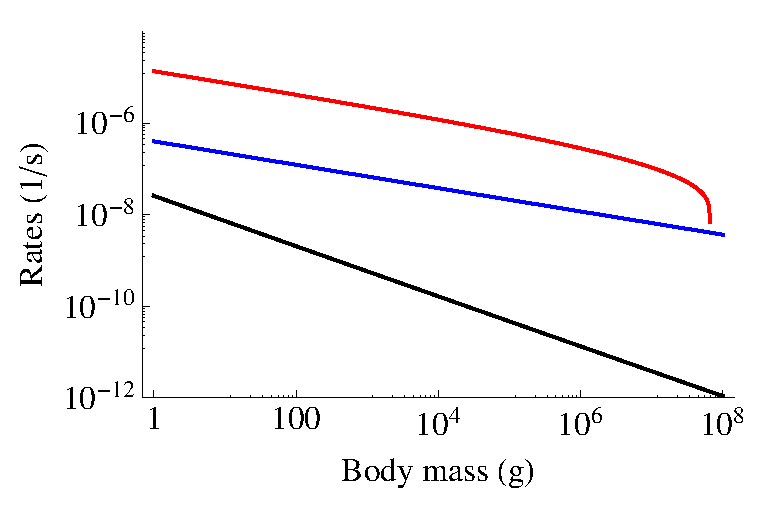
\includegraphics[width=0.4\textwidth]{mortality-rate-comparison.eps}
\caption{\small{The rates of reproduction $\lambda$ (blue), starvation-based mortality $\mu$ (red), and survivorship-based death $\bar{d}$ (black) as a function of adult mass.}\label{fig:ratescomp}}
\end{figure}

We are interested in the specific death rate of the form $\dot{F}=-dF$, and using the derivative of Equation \ref{gompertz} we find that $d=c_{0}e^{c_{1}t}$. Our model considers the average rates over a population and lifecycle and the average death rate is given by 
\begin{eqnarray}
\bar{d}&=&\frac{1}{t_{\text{exp}}}\int_{0}^{t_{\text{exp}}}c_{0}e^{c_{1}t} dt \\
&=&\frac{c_{0}\left(e^{c_{1} t_{\text{exp}}}-1\right)}{c_{1}t_{\text{exp}}}
\end{eqnarray}
where $t_{\text{exp}}$ is the expected lifespan following the allometry of $t_{\text{exp}}=a_{2}M^{b_{2}}$ with $a_{2}=4.04\times10^{6}$ (s g$^{-b_{2}}$) and $b_{2}=0.30$ ~\cite{damuth1982analysis,calder1984}. Given the allometries above we have that
\begin{equation}
\bar{d}=\frac{a_{0} \left(e^{a_{1}a_{2}M^{b_{1}+b_{2}}}-1\right) M^{b_{0}-b_{1}-b_{2}}}{a_{1} a_{2}}
\end{equation}
which scales roughly like $M^{b_{0}}$ because $b_{1}$ and $b_{2}$ are close in value but opposite in sign. In Figure S\ref{fig:ratescomp} we compare the value of $\bar{d}$ to the reproductive, $\lambda$, and starvation-based mortality, $\mu$, rates. The values of $\bar{d}$ are orders of magnitude smaller than these rates for all mammalian masses, and thus, adding this non-starvation based death rate to our model does not shift our results within numerical confidence. 

{\bf NSM and the energy equivalence hypothesis}

The energy equivalence hypothesis is based on the observation that if one assumes that the total metabolism of an ecosystem $B_{\rm tot}$ is equally partitioned between all species ($B_{i}$, the total metabolism of one species, is a constant), then the abundances should follow $N\left(M\right)B\left(M\right)=B_{i}$ implying that $N\left(M\right)\propto M^{-\eta}$, where $\eta$ is the metabolic scaling exponent \citep{allen2002,enquist1998}. As $\eta \approx 3/4$ this hypothesis is consistent with Damuth's law \citep{allen2002}. However, the actual equivalence of energy usage of diverse species has not been measured at the population level for a variety of whole populations. Figure S\ref{fig:equivalence} recasts the results of the NSM in terms of this hypothesis and shows that $F^{*}B$ is nearly constant over the same range of mammalian sizes up to the asymptotic behavior for the largest terrestrial mammals. 

\begin{figure}[h!]
\centering
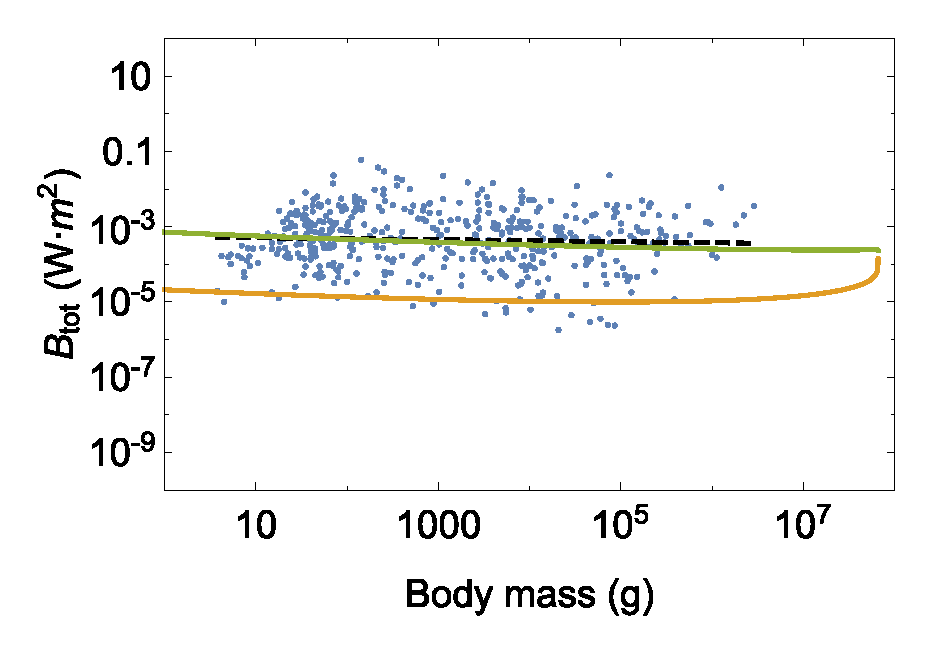
\includegraphics[width=0.4\textwidth]{fig_FPenergyequiv.eps}
\caption{\small{ Total energetic use $B_{\rm tot}$ of consumer populations at the steady state as a function of body mass ($F^*$ is shown in green and $H^*$ in orange).  The data are from Damuth \citep{Damuth:1987kr} and have been converted to
  total population metabolism using the allometric relationships for
  metabolic rate (e.g. Refs.~\citep{West:2001bv,hou,moses2008rmo}).}\label{fig:equivalence}}
\end{figure}

{\bf Application of NSM limits to aquatic mammals}
A theoretical upper bound on mammalian body size is given by $\epsilon_\sigma=0$, where mammals are entirely composed of metabolic reserves, and this occurs at $M=8.3\times 10^8$ (g), or $120$ times the mass of a male African elephant. We note this particular limit as it may have future relevance to considerations of the ultimate constraints on aquatic mammals.


\def\bibfont{\footnotesize}


% \bibliography{aa_starving_supplement}
\begin{thebibliography}{10}
\expandafter\ifx\csname url\endcsname\relax
  \def\url#1{\texttt{#1}}\fi
\expandafter\ifx\csname urlprefix\endcsname\relax\def\urlprefix{URL }\fi
\providecommand{\bibinfo}[2]{#2}
\providecommand{\eprint}[2][]{\url{#2}}

\bibitem{Kempes:2012hy}
\bibinfo{author}{Kempes, C.~P.}, \bibinfo{author}{Dutkiewicz, S.} \&
  \bibinfo{author}{Follows, M.~J.}
\newblock \bibinfo{title}{{Growth, metabolic partitioning, and the size of
  microorganisms.}}
\newblock \emph{\bibinfo{journal}{PNAS}} \textbf{\bibinfo{volume}{109}},
  \bibinfo{pages}{495--500} (\bibinfo{year}{2012}).

\bibitem{kempes2014morphological}
\bibinfo{author}{Kempes, C.~P.}, \bibinfo{author}{Okegbe, C.},
  \bibinfo{author}{Mears-Clarke, Z.}, \bibinfo{author}{Follows, M.~J.} \&
  \bibinfo{author}{Dietrich, L.~E.}
\newblock \bibinfo{title}{Morphological optimization for access to dual
  oxidants in biofilms}.
\newblock \emph{\bibinfo{journal}{Proceedings of the National Academy of
  Sciences}} \textbf{\bibinfo{volume}{111}}, \bibinfo{pages}{208--213}
  (\bibinfo{year}{2014}).

\bibitem{West:2001bv}
\bibinfo{author}{West, G.~B.}, \bibinfo{author}{Brown, J.~H.} \&
  \bibinfo{author}{Enquist, B.~J.}
\newblock \bibinfo{title}{{A general model for ontogenetic growth}}.
\newblock \emph{\bibinfo{journal}{Nature}} \textbf{\bibinfo{volume}{413}},
  \bibinfo{pages}{628--631} (\bibinfo{year}{2001}).

\bibitem{moses2008rmo}
\bibinfo{author}{Moses, M.~E.} \emph{et~al.}
\newblock \bibinfo{title}{{Revisiting a model of ontogenetic growth: Estimating
  model parameters from theory and data}}.
\newblock
  \emph{\bibinfo{journal}{http://dx.doi.org.proxy.lib.sfu.ca/10.1086/679735}}
  \textbf{\bibinfo{volume}{171}}, \bibinfo{pages}{632--645}
  (\bibinfo{year}{2008}).

\bibitem{hou}
\bibinfo{author}{Hou, C.} \emph{et~al.}
\newblock \bibinfo{title}{{Energy uptake and allocation during ontogeny}}.
\newblock \emph{\bibinfo{journal}{Science}} \textbf{\bibinfo{volume}{322}},
  \bibinfo{pages}{736--739} (\bibinfo{year}{2008}).

\bibitem{pirt}
\bibinfo{author}{Pirt, S.}
\newblock \bibinfo{title}{The maintenance energy of bacteria in growing
  cultures}.
\newblock \emph{\bibinfo{journal}{Proceedings of the Royal Society of London B:
  Biological Sciences}} \textbf{\bibinfo{volume}{163}},
  \bibinfo{pages}{224--231} (\bibinfo{year}{1965}).

\bibitem{Heijnen}
\bibinfo{author}{Heijnen, J.} \& \bibinfo{author}{Roels, J.}
\newblock \bibinfo{title}{A macroscopic model describing yield and maintenance
  relationships in aerobic fermentation processes}.
\newblock \emph{\bibinfo{journal}{Biotechnology and Bioengineering}}
  \textbf{\bibinfo{volume}{23}}, \bibinfo{pages}{739--763}
  (\bibinfo{year}{1981}).

\bibitem{peters1986ecological}
\bibinfo{author}{Peters, R.~H.}
\newblock \emph{\bibinfo{title}{The Ecological Implications of Body Size}},
  vol.~\bibinfo{volume}{2} (\bibinfo{publisher}{Cambridge University Press},
  \bibinfo{address}{Cambridge}, \bibinfo{year}{1986}).

\bibitem{blueweiss1978relationships}
\bibinfo{author}{Blueweiss, L.} \emph{et~al.}
\newblock \bibinfo{title}{Relationships between body size and some life history
  parameters}.
\newblock \emph{\bibinfo{journal}{Oecologia}} \textbf{\bibinfo{volume}{37}},
  \bibinfo{pages}{257--272} (\bibinfo{year}{1978}).

\bibitem{stryer}
\bibinfo{author}{Stryer, L.}
\newblock \emph{\bibinfo{title}{{Biochemistry, Fourth Edition}}}
  (\bibinfo{publisher}{W.H. Freeman and Company}, \bibinfo{address}{New York},
  \bibinfo{year}{1995}).

\bibitem{Dunbrack:1993ec}
\bibinfo{author}{Dunbrack, R.~L.} \& \bibinfo{author}{Ramsay, M.~A.}
\newblock \bibinfo{title}{{The Allometry of Mammalian Adaptations to Seasonal
  Environments: A Critique of the Fasting Endurance Hypothesis}}.
\newblock \emph{\bibinfo{journal}{Oikos}} \textbf{\bibinfo{volume}{66}},
  \bibinfo{pages}{336--342} (\bibinfo{year}{1993}).

\bibitem{Lindstedt:1985hm}
\bibinfo{author}{Lindstedt, S.~L.} \& \bibinfo{author}{Boyce, M.~S.}
\newblock \bibinfo{title}{{Seasonality, Fasting Endurance, and Body Size in
  Mammals}}.
\newblock \emph{\bibinfo{journal}{Am. Nat.}} \textbf{\bibinfo{volume}{125}},
  \bibinfo{pages}{873--878} (\bibinfo{year}{1985}).

\bibitem{Lindstedt:2002td}
\bibinfo{author}{Lindstedt, S.~L.} \& \bibinfo{author}{Schaeffer, P.~J.}
\newblock \bibinfo{title}{{Use of allometry in predicting anatomical and
  physiological parameters of mammals.}}
\newblock \emph{\bibinfo{journal}{Lab. Anim.}} \textbf{\bibinfo{volume}{36}},
  \bibinfo{pages}{1--19} (\bibinfo{year}{2002}).

\bibitem{estermann}
\bibinfo{author}{Estermann, B.~L.}, \bibinfo{author}{Wettstein, H.-R.},
  \bibinfo{author}{Sutter, F.} \& \bibinfo{author}{Kreuzer, M.}
\newblock \bibinfo{title}{Nutrient and energy conversion of grass-fed dairy and
  suckler beef cattle kept indoors and on high altitude pasture}.
\newblock \emph{\bibinfo{journal}{Animal Research}}
  \textbf{\bibinfo{volume}{50}}, \bibinfo{pages}{477--493}
  (\bibinfo{year}{2001}).

\bibitem{michaletz2014convergence}
\bibinfo{author}{Michaletz, S.~T.}, \bibinfo{author}{Cheng, D.},
  \bibinfo{author}{Kerkhoff, A.~J.} \& \bibinfo{author}{Enquist, B.~J.}
\newblock \bibinfo{title}{Convergence of terrestrial plant production across
  global climate gradients}.
\newblock \emph{\bibinfo{journal}{Nature}} \textbf{\bibinfo{volume}{512}},
  \bibinfo{pages}{39--43} (\bibinfo{year}{2014}).

\bibitem{damuth1987interspecific}
\bibinfo{author}{Damuth, J.}
\newblock \bibinfo{title}{Interspecific allometry of population density in
  mammals and other animals: the independence of body mass and population
  energy-use}.
\newblock \emph{\bibinfo{journal}{Biological Journal of the Linnean Society}}
  \textbf{\bibinfo{volume}{31}}, \bibinfo{pages}{193--246}
  (\bibinfo{year}{1987}).

\bibitem{calder1984}
\bibinfo{author}{Calder, W.~A.}
\newblock \emph{\bibinfo{title}{Size, function, and life history}}
  (\bibinfo{publisher}{Harvard University Press}, \bibinfo{year}{1984}).

\bibitem{damuth1982analysis}
\bibinfo{author}{Damuth, J.}
\newblock \bibinfo{title}{Analysis of the preservation of community structure
  in assemblages of fossil mammals}.
\newblock \emph{\bibinfo{journal}{Paleobiology}} \textbf{\bibinfo{volume}{8}},
  \bibinfo{pages}{434--446} (\bibinfo{year}{1982}).

\bibitem{allen2002}
\bibinfo{author}{Allen, A.~P.}, \bibinfo{author}{Brown, J.~H.} \&
  \bibinfo{author}{Gillooly, J.~F.}
\newblock \bibinfo{title}{{Global biodiversity, biochemical kinetics, and the
  energetic-equivalence rule}}.
\newblock \emph{\bibinfo{journal}{Science}} \textbf{\bibinfo{volume}{297}},
  \bibinfo{pages}{1545--1548} (\bibinfo{year}{2002}).

\bibitem{enquist1998}
\bibinfo{author}{Enquist, B.~J.}, \bibinfo{author}{Brown, J.~H.} \&
  \bibinfo{author}{West, G.~B.}
\newblock \bibinfo{title}{{Allometric scaling of plant energetics and
  population density}}.
\newblock \emph{\bibinfo{journal}{Nature}} \textbf{\bibinfo{volume}{395}},
  \bibinfo{pages}{163--165} (\bibinfo{year}{1998}).

\bibitem{Damuth:1987kr}
\bibinfo{author}{Damuth, J.}
\newblock \bibinfo{title}{{Interspecific allometry of population density in
  mammals and other animals: the independence of body mass and population
  energy-use}}.
\newblock \emph{\bibinfo{journal}{Biol. J. Linn. Soc.}}
  \textbf{\bibinfo{volume}{31}}, \bibinfo{pages}{193--246}
  (\bibinfo{year}{1987}).

\end{thebibliography}



% \end{bibunit}



\end{document}
